\documentclass[12pt,french, a4paper]{report}

% This is the main framework I use for my LateX documents.
% main.tex by Alexis GRACIAS

%%%%%%%%%%%%%
% LIBRARIES %
%%%%%%%%%%%%%

\usepackage{babel}
\usepackage{hyperref} % Add links to the table of content, files and website
\usepackage{graphicx} % Required for inserting images
\usepackage{tabto}
\usepackage[dvipsnames]{xcolor} % Text color package and more colors
\usepackage{tikz} % Graph package
\usepackage{pdfpages}
\usepackage{caption}
\usepackage{subcaption}
%\usepackage[demo]{graphicx}
\usepackage[utf8]{inputenc}
\usepackage{amsmath,amsfonts,mathtools,stmaryrd} % Math libraries

\usepackage{listings} % required for specific languages
\lstset{ % Set listing package options
    language=bash, % choose the language of the code
    basicstyle=\fontfamily{pcr}\selectfont\footnotesize\color{red},
    keywordstyle=\color{black}\bfseries, % style for keywords
    numbers=none, % where to put the line-numbers
    numberstyle=\tiny, % the size of the fonts that are used for the line-numbers     
    backgroundcolor=\color{white},
    showspaces=false, % show spaces adding particular underscores
    showstringspaces=false, % underline spaces within strings
    showtabs=false, % show tabs within strings adding particular underscores
    frame=single, % adds a frame around the code
    tabsize=2, % sets default tabsize to 2 spaces
    rulesepcolor=\color{gray},
    rulecolor=\color{black},
    captionpos=b, % sets the caption-position to bottom
    breaklines=true, % sets automatic line breaking
    breakatwhitespace=false, 
}

%\usepackage{eso-pic,lipsum}
%\AddToShipoutPicture{%
%	\AtTextCenter{%
%		\fboxsep5mm \fboxrule=0.8pt
%		\makebox(0,0)[c]{\fbox{\rule{0pt}\textheight\rule\textwidth{0pt}}}%
%	}%
%}

%%%%%%%%%%%%
% COMMANDS %
%%%%%%%%%%%%

\lstset{aboveskip=\baselineskip,belowskip=\baselineskip,basicstyle=\ttfamily} % Formating line break after bash commands

% Get rid of 0. chapter's number
\makeatletter 
\renewcommand{\thesection}{%
  \ifnum\c@chapter<1 \@arabic\c@section
  \else \thechapter.\@arabic\c@section
  \fi
}
\makeatother

% Rules for \bar{x} and \overline{x} commands
\makeatletter
\newcommand*{\Xbar}{}%
\DeclareRobustCommand*{\Xbar}{%
  \mathpalette\@Xbar{}%
}

\newcommand*{\@Xbar}[2]{%
  % #1: math style
  % #2: unused (empty)
  \sbox0{$#1\mathrm{X}\m@th$}%
  \sbox2{$#1X\m@th$}%
  \rlap{%
    \hbox to\wd2{%
      \hfill
      $\overline{%
        \vrule width 0pt height\ht0 %
        \kern\wd0 %
      }$%
    }%
  }%
  \copy2 %
}
\makeatother

%%%%%%%%%%%%%%%%%%%%%%
% DOCUMENTS SETTINGS %
%%%%%%%%%%%%%%%%%%%%%%
% Fist page
\title{\Huge Fiche de révision Droit}
\author{\LARGE Alexis GRACIAS}
\date{\Large \today}

% Document
\begin{document}
\maketitle
\Large \tableofcontents

%%%%%%%%%%%
% INCLUDE %
%%%%%%%%%%%

\chapter{Les normes et le raisonnement juridique}
\section{Hiérarchie des normes}
\subsection{Définition}
\large{
\textbf{Le droit} est un ensemble de \textbf{règles} qui organisent la vie en société et régissent \textbf{les relations entre les individus, les institutions et l'état.}
Ces règles sont créées par des \textbf{autorités compétentes}, comme le législateur, et sont appliquées par des tribunaux ou d'autres institutions de justice \newline

Le droit est divisé en plusieurs branches, comme : \newline

}
\begin{itemize}
    \item \textbf{Le droit civil} : concerne les relations entre les particuliers, par exemple en matière de mariage, de propriétés ou de contrats
    \item \textbf{Le droit pénal} : détermine les infractions (crimes, délits, contraventions) et fixe les sanctions applicables
    \item \textbf{Le droit administratif} : encadre les relations entre les citoyens et les administrations publiques
    \item \textbf{Le droit internationnal} : régit les relations entre les états et questions juridiques dépassant les frontières nationnales
    \item \textbf{Le droit commercial} : concerne les activités économiques, les entreprises et les transactions commerciales
\end{itemize}
En cas de non respect de ces règles, le citoyen encours des sanctions. Le droit peut évoluer dans le temps en fonction des changements sociaux, technologiques ou économiques
\begin{center}
    \begin{figure}[hbt!]
        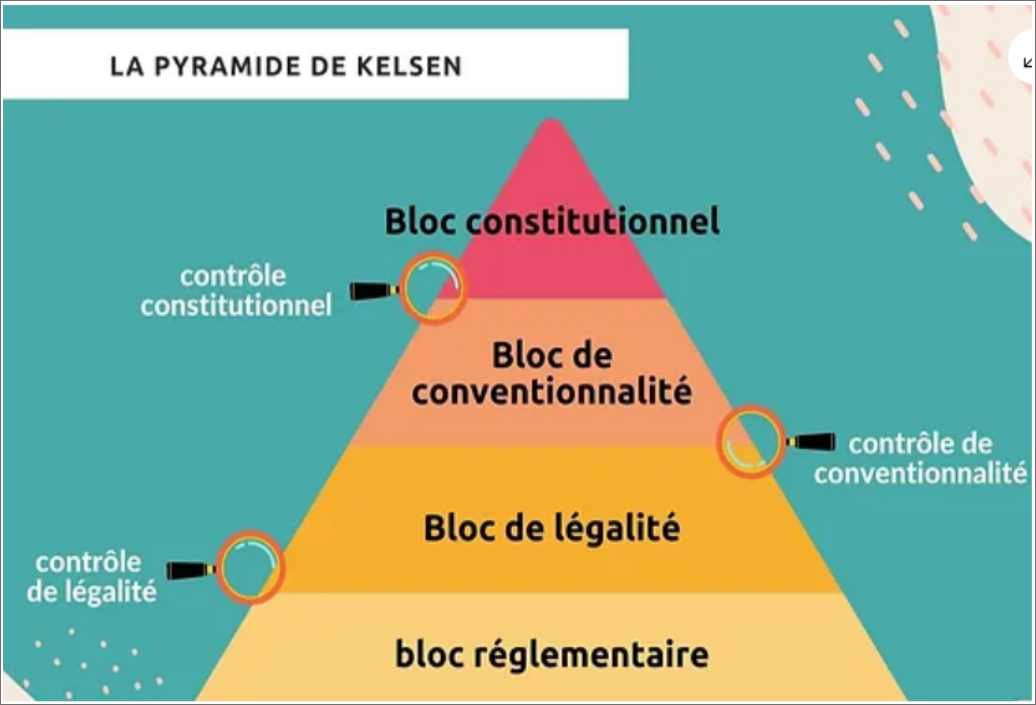
\includegraphics[scale=0.4]{Pics/Pyramide_de_Kelsen.png}
        \caption{Hiérarchie des normes}
    \end{figure}
\end{center}
\newpage
\section{Les normes}
Les \textbf{normes juridiques} sont à différentier des \textbf{normes sociales}. Une norme juridique est une règle qui établit une source de droits et d'obligations juridiques tandis
qu'une norme sociale provient d'une tradition, de la morale lorsqu'un individu se socialise. 
\subsection{Bloc constitutionnel}
C'est la Constitution : un ensemble de normes juridiques, de principes et de règles appliquées par le conseil constitutionnel. \footnote{Vérifie la conformité des lois à la Constitution}
\begin{center}
    \begin{figure}[hbt!]
        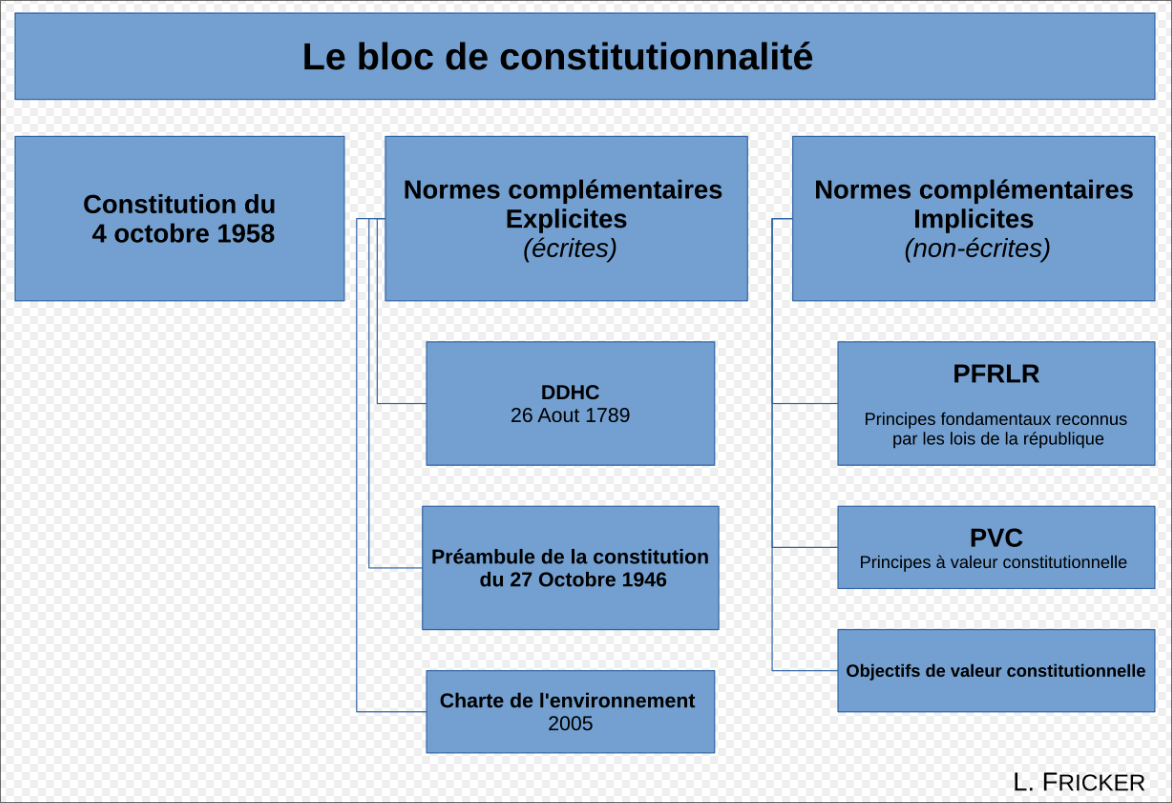
\includegraphics[scale=0.3]{Pics/Bloc_de_constitutionnalite.png}
        \caption{Bloc constitutionnel}
    \end{figure}
\end{center}
\newpage
\subsection{Bloc conventionnel}
\textbf{Le bloc de conventionnalité l'ensemble des traités et conventions entre les Etats ou entre mes Etats et les organisations internationnales} \newline
Exemple : l'\textbf{UE} est une organisation économique et politique qui rasssemble 27 états membres. Elle a pour but de promouvoir la paix, la stabilité et la coopération économique entre les états memebres. \newline
\begin{center}
    \begin{figure}[hbt!]
        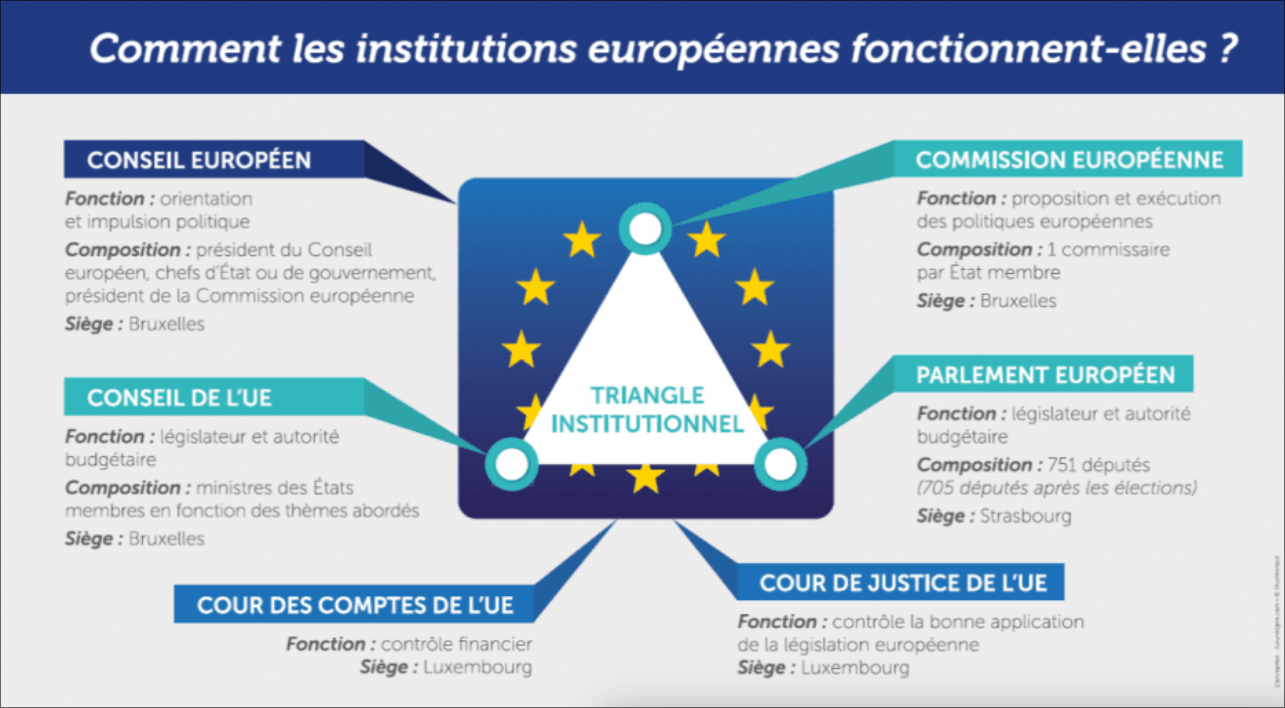
\includegraphics[scale=0.3]{Pics/Institutions_UE.png}
        \caption{Illustration des institutions dans l'Union Européenne}
    \end{figure}
\end{center}
\newpage



\end{document}
